\documentclass[a4paper]{article}

\usepackage[spanish]{babel} % Le indicamos a LaTeX que vamos a escribir en español.
\usepackage[utf8]{inputenc} % Permite utilizar tildes y eñes normalmente
\usepackage{caratula} % Se puede descargar en ~> https://github.com/bcardiff/dc-tex
\usepackage[font={small,it}]{caption}
%hopefully no floting images
\usepackage{floatrow}
\floatplacement{figure}{H}
\floatplacement{table}{H}

\begin{document} % Todo lo que escribamos a partir de aca va a aparecer en el documento.
%fran
%\sloppy

% Completar los datos de la caratula
\titulo{Implementación y evaluación de un TTS de habla con distos grados de acento extranjero} 
\fecha{\today}
\materia{}
\grupo{}

% Completar los integrantes del grupo:)
\integrante{Negri, Franco }{893/13}{franconegri2004@hotmail.com}

\maketitle

\tableofcontents

\pagebreak

\section{Introducción}

\noindent Un sistema de Text To Speech (TTS) es aquel que genera habla artificial a partir de un texto de entrada. En la actualidad estos sistemas se encuentran incluidos en muchas aplicaciones domesticas, desde navegación por GPS, asistentes personales inteligentes (como es el caso de SIRI), ayuda para personas no videntes, traducción automática, etc.

\noindent En las últimas décadas se han visto grandes progresos en este campo, siendo capaces de modelar con cierto grado de efectividad cuestiones tales como la prosodia del hablante, emociones, etc. Si bien actualmente se considera que el estado del arte para la síntesis es el entrenamiento con redes neuronales profundas (DNN), una técnica todavía utilizada es la que utiliza modelos ocultos de markov mas modelos de mezcla de gaussianas (HMM+GMM) que, a partir de un corpus de datos de entrenamiento, extrae información acústica y genera un modelo probabilístico que permita sintetizar habla. 

Consideramos que este método si bien no nos permitirá obtener la mejor voz posible, nos permitirá entender mejor los features con los que trabajamos y por lo tanto modificarlos según consideremos conveniente, algo que puede volverse mas complicado cuando se esta trabajando con redes neuronales profundas.

\noindent En este trabajo de tesis se estudia una manera posible de generar un TTS basado en HMMs capaz de sintetizar habla en español con acento extranjero. Las razones por las que podría querer diseñarse un sistema con estas características varían desde un punto de vista puramente técnico, ya que un sistema así permitiría la utilización de corpus de entrenamiento de hablantes no nativos para la generación de una nueva voz, pasando por cuestiones lingüísticas, como es poder vislumbrar el limite en que un acento deja de parecernos local para pasar a ser extranjero y cuestiones psicológicas: lograr distintos efectos sobre el usuario, quien podría reaccionar distinto ante diferentes acentos.

\noindent En el transcurso de este trabajo se espera además evaluar la prosodia y la fonética del modelo generado con estas características, como así también evaluar su inteligibilidad. Además pretenderemos evaluar la efectividad de técnicas de speaker adaptation cuando se utilizan corpus de distintas nacionalidades con repertorios fonéticos disimiles (para este caso de estudio: castellano e ingles)

\noindent Para este trabajo nos basaremos fuertemente en la síntesis/análisis mel-cepstral, speech parameter modeling usando HMMs y speech parameter generation usando HMMs, como es descripto en la disertación doctoral \textit{Simultaneous Modeling of phonetic and prosodic parameters, and characteristic conversion for hmm-based text-to-speech systems} del Profesor Tadashi Kitamura, Nagoya Institute of Technology\cite{phoneticAndProsodic}.


Como introducción a este trabajo comenzaremos analizando las decisiones de metodología utilizadas a lo largo de la investigación, así también como detalles teóricos como el mapeo de fonemas necesario para adaptar el repertorio fonético del ingles al castellano, etc.

En las siguiente secciones se detallaran distintos temas que fueron necesarios abordar para llevar a cabo esta tesis. En orden de aparición estos son:

\begin{enumerate}
\item Realizar un etiquetado fonético de distintos corpus de audios.

\item Realizar un mapeo entre los fonos del castellano y los del ingles. Estos serán necesarios en el paso siguiente donde será requerimiento indispensable tener modelados los mismos fonos para todos los modelos.

\item Realizar el entrenamiento de los HMM+GMM. Para esto contaremos con el framework de modelado de HMMs HTS. 

\item Utilizar las herramientas provistas por HTS para interpolar entre modelos y poder sintetizar habla con distintos grados de fonética y prosodia inglesa.

\end{enumerate}

Para finalizar el apartado teórico discutiremos algunos aspectos implémentatelos de HTS y las otras herramientas utilizadas en este trabajo.

\pagebreak
\section{Metodología}
\section{Objetivos}

El objetivo de este trabajo se sentrará generar un sistema de sintesis de habla basado en HMMs que sea capaz de sintetizar habla en español con acento extranjero. Una vez obtenidos resultados que consideremos aceptables, procederemos a una etapa de experimentación donde buscaremos \completarObjetivos

\break

\section{Metodología}

En esta sección presentaremos la metodología utilizada para la generación de HMMs, la interpolación entre los mismos y otras tecnicas utilizadas.


A modo de resumen, estos serán los pasos a realizar:


A partir de tres corpus de datos, dos de ellos en castellano y uno en ingles, se realizará un etiquetado fonetico de los corpus para su posterior utilización en el entrenamiento de los HMMs.


Realizar el entrenamiento del sistema. Para esto contaremos con un sistema de sintesis de voz basado en HMM conocido como HTS. 


Una vez generados los HMMs (Uno por cada corpus disponible) utilizaremos herramientas provistas por HTS para interpolar entre ellos y así obtener distintos grados de fonetica y prosodia inglesa a la hora de sintetizar audios.


Dado que el castellano y el ingles no utilizan los mismos simbolos foneticos, si queremos sintetizar audios en castellano con el HMM generado con el corpus en ingles, un desafío que deberemos resolver es el de cubrir todos los simbolos foneticos del castellano por alguno del ingles.

\subsection{Preparación De los datos}


Como ya adelantamos, en este trabajo contamos con tres corpus de datos dispoinbles:


\begin{itemize}
\item secyt-mujer: 741 oraciones, $48$ minutos de habla.
\item loc1\_pal: 1593 oraciones, $2$ horas y $26$ minutos de habla.
\item CMU-ARCTIC-SLT: 1132 oraciones, 56 minutos de habla.
\end{itemize}


Dadas la cantidad de horas de audio disponibles, tanto para loc1\_pal como para CMU-ARCTIC-SLT decidimos utilizar alineamiento forzado para obtener las transcripciones foneticas necesarias para el entrenamiento. Para esto se utilizó Festival y Festvox que a partir de los audios y sus transcripciones grafemicas, permite realizar EHMM alignment sobre el corpus de datos. Para secyt-mujer contabamos previamente con las transcripciones foneticas ya realizadas por lo que decidimos utilizar estas. 


Por otra parte, festival nos permitirá generar features contextuales sobre cada fonema, como el fonema que lo precede, cantidad de palabras en la oración, si la silaba en la que se encuentra esta acentuada, etc. Mas adelante en este trabajo se explicará de que manera son utilizados estos features.


Para este trabajo todos los audios usarán sampling rate de 48kHz, precisión de 16 bits, mono.


% Cosas para hablar:
%TODO: phonetically balanced?
% contextual factors: cuales son, para que sirven.
% desarrollar generacion de uternaces: secty alineaminento mixto: tiempos a mano, features automaticos.
% el etiquetado de cmu\_arctic es en ingles y mapeando al castellano.

\subsection{Entrenamiento Con HTS}

Tanto para el entrenamiento y sintesis del habla se utilizará HTS.


Comenzaremos dando un pequeño resumen del funcionamiento del sistema utilizado:


HTS es un TTS que modela simultaneamente la duración, el espectro (mel-cepstrum) y la frecuencia principal (f0) de manera simultanea utilizando un framework de HMM:

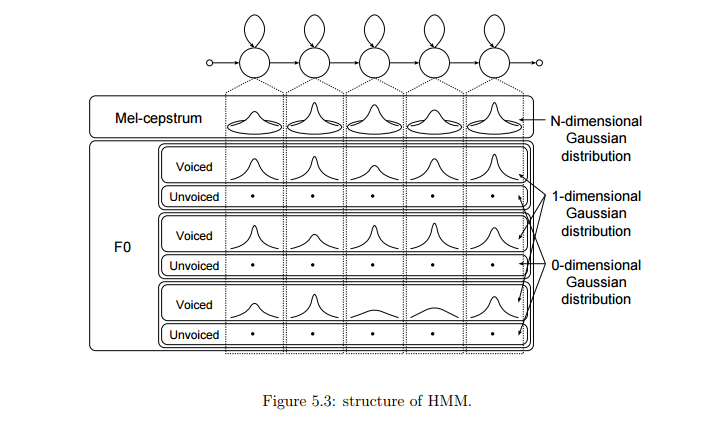
\includegraphics[scale=0.5]{imagenes/hmm.png}


Por otra parte HTS toma la decición de modelar la información prosodica dentro de este mismo framework. Para esto, las distribuciónes para el espectro, la frecuencia principal y las duraciónes son clusterizadas independientemente utilizando tecnicas de aprendisaje automatico y arboles de decición. A continuación se presenta una vista esquematica de la estructura de este nuevo hmm:

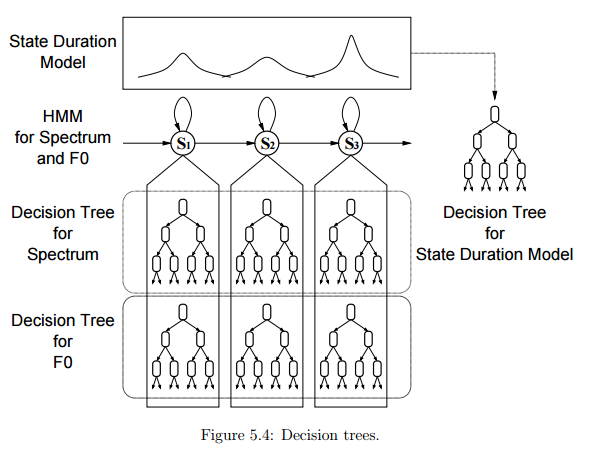
\includegraphics[scale=0.5]{imagenes/hmmContext.png}


En particular para este trabajo el entrenamiento de todos los modelos se realiza utilizando senones (5 fonemas) para los HMM generados.

% Cosas para hablar:
% 5 fonemas.
% hmms
% arboles de decición.
%questions

\subsection{Sintesis utilizando hts\_engine}


Para la sintesis se utilizó hts\_engine, una herramienta de linea de comandos que no solo permite sintetizar oraciones utilizando los modelos acusticos generados sino ademas interpolar entre los distintos HMMs disponibles. Utilizaremos esta herramienta para interpolar entre los HMMs de ingles y castellano para lograr nuevos modelos que mezclen los features acusticos con distintos grados de ingles y de castellano.

Un desafío que se presenta para este trabajo es el mapeo de los fonemas del ingles al castellano. Para empezar, la transcripcion fonetica realizada por festival de las oraciones en ingles puede utilizar 50 simbolos distintos, mientras que la transcripción fonetica del castellano utiliza 31. Habiendo ademas muchos simbolos sin equivalencia. (por ejemplo, con el fonema /rr).

Para resolver esto desarollamos una solución adhoc que consistió en desarrollar una función sobreyectiva que permita tener cubiertos los 31 fonemas del castellano por alguno del ingles.

% Cosas para hablar:
% mapeo utilizado mostrar.
% Expandir en que consiste la interpolación.
\pagebreak
\section{Experimentación}

En esta sección intentamos validar que el habla sintetizada por los modelos generados realmente puede ser identificada como perteneciente a personas de habla inglesa, y al mismo tiempo evaluar sus grados de inteligibilidad. Para eso se condujo una encuesta perceptual donde a cada participante se le presentó una oración sintetizada con distintos grados de mezcla de español e inglés y se le pidió que la transcribiera y que intentara identificar la nacionalidad del hablante. 

La encuesta se realizó a través de Internet, con el mismo set de instrucciones para todos los participantes y pidiendo como requisito la utilización de auriculares. Cada participante podía contestar un máximo de $5$ veces, presentándoles siempre oraciones distintas.

Nos propusimos como objetivo conseguir $5$ respuestas para cada uno de los $50$ audios sintetizados, momento en el cual se cerró la posibilidad de contestar. Se llevó a cabo desde el $18$ de octubre de $2017$ hasta el primero de diciembre del mismo año, tiempo durante el cual fue publicitada en distintas redes sociales y listas de emails de distintas facultades.

Con el objetivo de no influir en las respuestas de los participantes, se procuró darles la información mínima indispensable para completar la encuesta. Por este motivo, en ningún momento de la encuesta se especifica el objetivo real de la misma. Con la intención de homogeneizar la muestra, fue requisito obligatorio utilizar auriculares para la encuesta. También se le pidió a cada participante que la realizara en un lugar silencioso y tranquilo.

A continuación, describimos la forma en que se construyeron los audios usados en esta evaluación y la interfaz de la encuesta. Luego mostramos los datos demográficos  obtenidos. Más adelante, continuamos con un análisis exhaustivo de inteligibilidad y origen atribuido a las oraciones.
Por último, para evaluar la hipótesis original, compondremos estos dos ejes para dilucidar el grado de validez de los resultados.

\section{Audios sintetizados}

Para evitar que el participante pudiera deducir las palabras de los audios a partir de las palabras vecinas, las mismas fueron generadas de manera \textit{semánticamente impredecible}. Esto significa que a partir de una lista de sustantivos, adjetivos, determinantes y verbos se generaron oraciones de manera aleatoria con la siguiente estructura:

$$\textnormal{\textit{Determinante Adjetivo Sustantivo Verbo Determinante Sustantivo}}$$

Luego, para asegurarnos de estar cubriendo todos los posibles fonos del castellano, las oraciones fueron modificadas para ser fonéticamente balanceadas. Esto significa que incluimos entre cinco y diez veces cada fono perteneciente a una consonante (del castellano) y al menos veinte veces cada fono perteneciente a una vocal.

Los oraciones generadas fueron:

\begin{itemize}
\item Oración 1: Mi montaña aguileña recorrió la esquina.
\item Oración 2: Aquel fuerte vidrio prefirió aquel botón.
\item Oración 3: Este enjoyado juez comprará nuestro corchete.
\item Oración 4: Tu estrecho posavasos gritó la fechoría.
\item Oración 5: Nuestro nublado tigre concluyó a este chupetín.
\item Oración 6: Su profundo riñón apoyó a Julio.
\item Oración 7: El frío churrasco oyó lo de Polonia.
\item Oración 8: Las acongojadas cotorras sonrieron a mi círculo.
\item Oración 9: Ese gruñón perro prometió a esos cuñados.
\item Oración 10: El nudillo argentino perdió su vaso.
\end{itemize}

Para cada una de estas diez oraciones se varió el nivel de mezcla entre $30\%$ de inglés + $70\%$ castellano hasta $70\%$ de inglés + $30\%$ de castellano, con $10\%$ de incremento. De esta manera, para cada oración hay $5$ mezclas diferentes, lo que hace un total de $50$ audios sintetizados diferentes.

\section{Interfaz}\label{interfaz}

En esta sección se presenta la interfaz utilizada para realizar la encuesta junto con las decisiones de diseño más relevantes. En la Figura \ref{personalData} se presenta la página con la que todos los participantes fueron recibidos. A fin de conocer de manera general la demografía encuestada, a cada participante se le pidió que indicara el rango correspondiente a su edad, yendo desde $18$ a $25$, $26$ a $35$, y así de diez en diez.

\begin{figure}[htp]
\begin{center}
\fbox{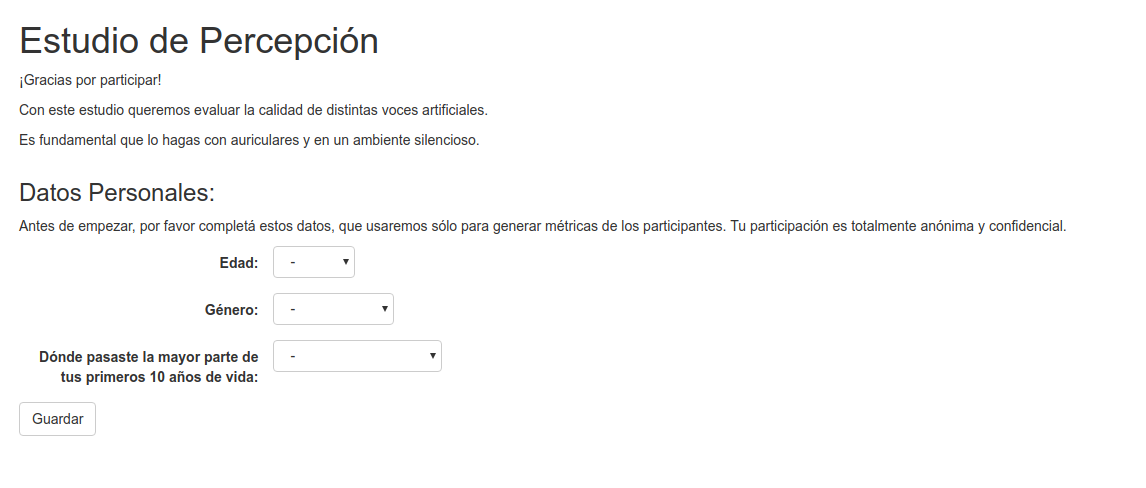
\includegraphics[scale=0.6]{estudio_online/estudio1.png}}
\end{center}
\caption{Primera pantalla de la encuesta, en la cual se recaban datos personales}
\label{personalData}
\end{figure}

Se le pidió, además, que indicara su género: ``masculino'', ``femenino'', ``otro'', ``no contesta'' y la provincia donde pasó la mayor parte de sus primeros diez años de vida. Consideramos que estos datos son importantes para el estudio ya que dependiendo de ellos los resultados variarán indefectiblemente. Por ejemplo la transcripción que obtendremos de un participante de $50$ años de Capital Federal será distinta a la de alguien de $18$ años de Córdoba. El diferente uso de los alofonos, modismos y variantes prosódicas y capacidades auditivas jugarán un papel importante en la interpretación de la oración y la apreciación del origen del hablante.

\begin{figure}
\begin{center}
\fbox{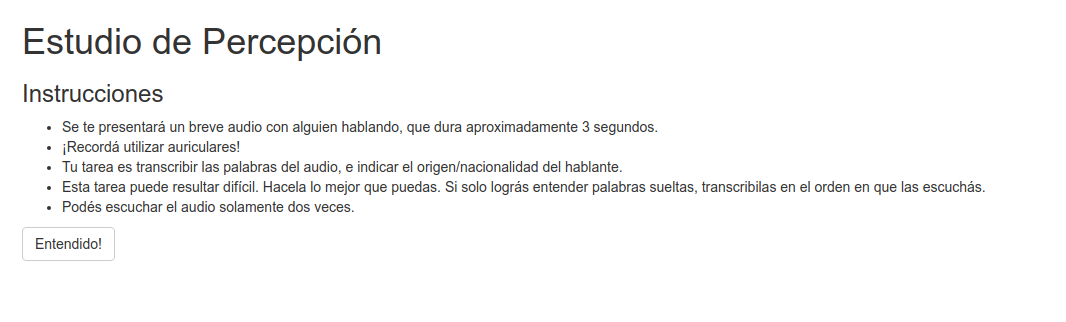
\includegraphics[scale=0.6]{estudio_online/estudio2.png}}
\end{center}
\caption{Pantalla con las instrucciones de la encuesta}
\label{instrucciones}
\end{figure}

Como puede verse en la Figura \ref{instrucciones}, una vez completados estos datos, a cada participante se le presentó otra vista con las instrucciones específicas para completar la encuesta. Una vez presionado el botón de ``Entendido!'' se les presentó el primer audio, que podían escuchar un máximo de $2$ veces, una caja de texto libre donde ingresar la transcripción del mismo y una caja de texto libre donde podían escribir cual consideraban que era el origen de la nacionalidad correspondiente a la voz, como puede apreciarse en la Figura \ref{transcripcion}.

\begin{figure}
\begin{center}
\fbox{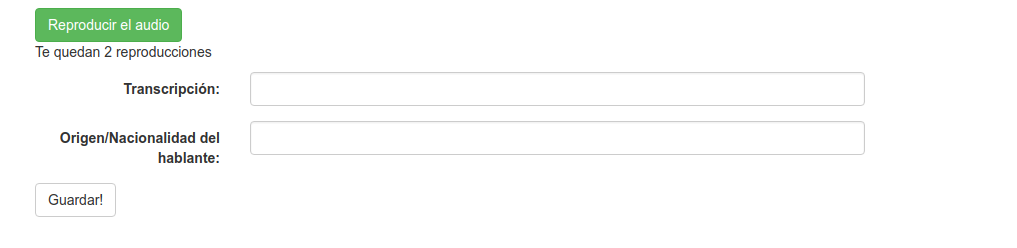
\includegraphics[scale=0.6]{estudio_online/estudio3.png}}
\end{center}
\caption{Pantalla de transcripción}
\label{transcripcion}
\end{figure}

Una vez guardada la respuesta, se le preguntó si quería continuar transcribiendo otro audio. En caso de haber completado cinco audios, se le mostró un mensaje indicando que ya podía cerrar la encuesta:

\begin{center}
\fbox{
¡Muchas gracias por tu participación! Ya podés cerrar la ventana del navegador.}
\end{center}

\pagebreak
\section{Trabajo Futuro}

Como fue discutido en la sección de experimentación, una interpolación general puede producir que ciertos fonemas se alejen demasiado del fonema real del castellano, disminuyendo la inteligibilidad de la voz sintetizada. Un posible camino a seguir es realizar una interpolación controlada que permita regular cada fonema por separado. Para fonemas que puedan resultar problematicos como el caso de la /r bibrante el grado de interpolación podría dejarse mas cercano al castellano, mientras que para fonemas con comportamientos mas similares el grado de interpolación podría llevarse mas cerca del modelo ingles.

%expandir
\pagebreak
\section{Apendice}

\section{Transcripciones ingresadas por los participantes} \label{transcripcionesParticipantes}

\noindent Oraciones originales:
\begin{multicols}{2}
\let\mcnewpage=\newpage
\makeatletter
\renewcommand\newpage{%
    \if@firstcolumn
        \hrule width\linewidth height0pt
        \columnbreak
    \else
        \mcnewpage
    \fi
}
\makeatother
\tiny
\centering
\begin{supertabular}{|c|c|}
\hline
#Oración& Transcripción\\
\hline
1&Mi montaña aguileña recorrió la esquina\\
\hline
2&Aquel fuerte vidrio prefirió aquel botón\\
\hline
3&Este enjoyado juez comprará nuestro corchete\\
\hline
4&Tu estrecho posavasos gritó la fechoría\\
\hline
5&Nuestro nublado tigre concluyó a este chupetín\\
\hline
6&Su profundo riñón apoyó a Julio\\
\hline
7&El frío churrasco oyó lo de Polonia\\
\hline
8&Las acongojadas cotorras sonrieron a mi círculo\\
\hline
9&Ese gruñón perro prometió a esos cuñados\\
\hline
10&El nudillo argentino perdió su vaso\\
\hline
\end{supertabular}
\end{multicols}

\noindent Transcripciones: Oración, Mezcla de ingles, Origen, Transcripción

\begin{multicols}{2}
\let\mcnewpage=\newpage
\makeatletter
\renewcommand\newpage{%
    \if@firstcolumn
        \hrule width\linewidth height0pt
        \columnbreak
    \else
        \mcnewpage
    \fi
}
\makeatother
\tiny
\centering
\begin{supertabular}{|p{0.1cm}|p{0.1cm}|p{2cm}|p{3.7cm}|}
\hline
1&30&	Argentina&	Mi montaña aguileña recorrió la esquina	\\
\hline
1&30&	Argentino&	Mi montaña aguileña recorrio la esquina	\\
\hline
1&30&	española&	mi montaña aguileña recorrió la esquina	\\
\hline
1&30&	Norte argentino&	Mi montaña aguileña recorrió la esquina	\\
\hline
1&30&	argentina&	mi montania aguilenia recorrió la esquina	\\
\hline
1&30&	Latino&	Mi montaña aguileña recorrió la esquina	\\
\hline
1&40&	Español&	Mi montaña aguileña recorrió la esquina	\\
\hline
1&40&	Ingles&	MI montaña aguileña recorrió la esquina	\\
\hline
1&40&	Uruguay&	Mi montaña recorrió la esquina	\\
\hline
1&40&	Argentina&	mi montaña aguileña recorrió la esquina	\\
\hline
1&40&	centroamerica&	Mi montaña aguileña recorrió la esquina	\\
\hline
1&40&	estadounidense&	mi montaña aguileña recorrio la esquina	\\
\hline
1&40&	EEUU&	Mi montaña aguileña recorrió la esquina	\\
\hline
1&50&	Boliviana&	Mi montaña recorrio la esquina	\\
\hline
1&50&	EEUU hablando español&	mi montaña milenia recorrió la esquina	\\
\hline
1&50&	Inglés&	Mi montaña aguileña recorrio la esquina	\\
\hline
1&50&	Japonés&	Recorrio la esquina	\\
\hline
1&50&	norteamericana&	mi montaña aguileña recorrió la esquina	\\
\hline
1&50&	Inglesa&	mi montaña pedigüeña recorrió la esquina	\\
\hline
1&50&	Estadounidense&	mi montaña aguileña recorrio la esquina	\\
\hline
1&50&	Estadounidense&	mi montaña aguileña recorrió la esquina	\\
\hline
1&60&	estadounidense&	Mi montaña aguileña recorrió la esquina	\\
\hline
1&60&	Estados unidos&	Mi montaña aguilenia recorrió la esquina	\\
\hline
1&60&	Irlanda&	Mi montaña aguileña recorrió la esquina.	\\
\hline
1&60&	Norte argentino&	Mi montaña aguileña recorrió la esquina	\\
\hline
1&60&	catellano&	recorriendo la esquiena	\\
\hline
1&60&	EEUU&	mi montaña aguileña recorrió la esquina	\\
\hline
1&60&	No se especifica&	Mi montaña..... recorrió la esquina	\\
\hline
1&60&	eeuu&	mi montaña aguileña recorrió la esquina	\\
\hline
1&60&	frances&	mi montaña recorrió la esquina	\\
\hline
1&70&	Ninguna&	Mi monzonia la cigüeña recorrio la esquina	\\
\hline
1&70&	Italiano&	Corrio a la esquina	\\
\hline
1&70&	Castellano&	Recorrió la esquina	\\
\hline
1&70&	Guam&	Mí montoña aguileña recorrió la esquina	\\
\hline
1&70&	Canadá&	Mi montaña aguileña recorrió la esquina	\\
\hline
1&70&	EEUU&	Mi corrió la esquina	\\
\hline
1&70&	nose&		\\
\hline
2&30&	argentino&	Aquel fuerte vidrio prefirió aquel botón	\\
\hline
2&30&	Ninguna&	Aquel fuerte vidrio prefirio aquel boton	\\
\hline
2&30&	Ninguna&	Aquel fuerte vidrio prefirió aquel botón	\\
\hline
2&30&	Argentino&	aquel fuerte vidrio prefirio aquel boton	\\
\hline
2&30&	Chile&	aquel fuerte vidrio prefirió aquel botón	\\
\hline
2&30&	Argentina&	aquel fuerte vidrio prefirió aquel botón	\\
\hline
2&40&	Espa;ol&	Aquel fuerte vidrio prefirio aquel boton	\\
\hline
2&40&	Ingles&	Aquie fuerte vidrio prefirio aquel boton	\\
\hline
2&40&	Argentino&	Aquel fuerte vidrio prefirio aquel boton	\\
\hline
2&40&	Norte argentino&	Aquel fuerte vidrio prefirió aquel botón	\\
\hline
2&40&	centroamericana&	aquel fuerte vidrio prefirió aquel boton	\\
\hline
2&40&	argentina&	aquel fuerte vidrio percibió al boton	\\
\hline
2&40&	Gallega&	Aquel fuerte vidrio prefirió aquel botón.	\\
\hline
2&50&	Inglesa&	Aqueo fuerte vidrio perforo aquel boton	\\
\hline
2&50&	paraguay&	aquel vidrio presiono aquel boton	\\
\hline
2&50&	francés&	aquél fuerte vidrio prefirió aquél botón	\\
\hline
2&50&	Estados Unidos&	aquel fuerte vidrio percibió aquel botón	\\
\hline
2&50&	EEUU&	Aquel fuerte vidrio prefirió aquel botón	\\
\hline
2&50&	Mexicano&	Aquel fuerte vidrio percibió aquel botón	\\
\hline
2&60&	inglesa&	aquel fuerte vidrio presidió aquel botón	\\
\hline
2&60&	Santo Domingo&	Aquel Fuel de vidrio prefiere aquel boton	\\
\hline
2&60&	paraguay&	te voy a pegar un palazo en la nuca y romperte el orto	\\
\hline
2&60&	estadounidense&	prefirió el botón	\\
\hline
2&60&	China&		\\
\hline
2&70&	Ingles&		\\
\hline
2&70&	Estados unidos&	Preferido aquel boton	\\
\hline
2&70&	inglesa&	aquel blablaba prefirio aquel boton	\\
\hline
2&70&	No se especifica&	Aquel fuerte vidrio prefirió aquel botón	\\
\hline
2&70&	Ninguna, es un robot.&		\\
\hline
2&70&	EEUU&	Aquel fuerte vidrio prefirió aquel boton	\\
\hline
3&30&	Argentino&	Este enjollado puede comparar nuestro cochete	\\
\hline
3&30&	Argentina&	Este enfueyado fue comparado corchete	\\
\hline
3&30&	Español&	Corchete	\\
\hline
3&30&	Argentino capital federal&	Corchete	\\
\hline
3&30&	Robot&	Este enrollado fue comprado nuestro corchete	\\
\hline
3&30&	española&	este enjoyado juez comprará nuestro corchete	\\
\hline
3&30&	Paraguayo&	este enjoyado fue comprado este corchete	\\
\hline
3&30&	Argentino&	Este enfollado juez comprará nuestro corchete	\\
\hline
3&30&	Español&	Este enfollado fue comprar nuestro corchete	\\
\hline
3&30&	No se especifica&	Este enjoyado juez comprará nuestro corchete	\\
\hline
3&30&	Indefinida&	Este enjoyado fue comprado corchete	\\
\hline
3&40&	La Rioja, Argentina&	Este encollado encontrará nuestro corchete	\\
\hline
3&40&	Ninguna nacionalidad&	Este fue juez corchete	\\
\hline
3&40&	España&	este enfollado comprara nuestro corchete	\\
\hline
3&40&	Española&	este fue nuestro corchete	\\
\hline
3&40&	Español neutro&	este enjoyado juez comprará nuestro corchete	\\
\hline
3&50&	Boliviano&	Este juez comprara nuestro	\\
\hline
3&50&	anglo&	este enrollado corchete	\\
\hline
3&50&	Maracaibo&	Este enconchado puede comprado nuestro cohete	\\
\hline
3&50&	Colombiano/Venezolano&	Este enfollado fue encontrar nuestro corchete	\\
\hline
3&50&	No se&	Este enrollado fue encontrar nuestro coechete	\\
\hline
3&60&	Ninguna&	Este en...fue comprar nuestro corchete	\\
\hline
3&60&	Inglesa&	Este nuestro corchete	\\
\hline
3&60&	gallego&	este enfollado comprara nuestro corchete	\\
\hline
3&60&	Ingles&	Este enfollado juez comprara nuestro corchete	\\
\hline
3&60&	inglés&	compraran nuestro corchete	\\
\hline
3&60&	Español&	Este ??? pues comprará nuestro corchete	\\
\hline
3&60&	estadounidense o inglés&	este ... nuestro corchete	\\
\hline
3&60&	estadounidense&	este fue nuestro corchete	\\
\hline
3&60&	Argentino&	Esté nuestro corchete	\\
\hline
3&60&	americano (EEUU)&	estoy nuestro corchete	\\
\hline
3&60&	Desconocido&	Comprara nuestro corchete	\\
\hline
3&70&	alemania&	este enfollado fuescon cuero nuestro follete	\\
\hline
3&70&	Hablante nativo de inglés& 	este ..... fue ..... en nuestro corchete	\\
\hline
3&70&	estadounidense&	este vuestro corchete	\\
\hline
3&70&	Ruso&	este fue encontrado con nuestro coche	\\
\hline
3&70&	estadounidense&	nuestro corchete	\\
\hline
4&30&	Argentina&	Tu estrecho posa basos grito la fechoria	\\
\hline
4&30&	Argentina&	Tu estrecho posa vasos grito	\\
\hline
4&30&	Cigbord&	Gritemos portavasos gritona fechoria	\\
\hline
4&30&	parece& una voz artificial	Tu estrecho posavasos gritó la fechoría	\\
\hline
4&30&	españa&	tu estrecho posavasos gritó la fechoría	\\
\hline
4&30&	Española&	Tu estrecho posavasos gritó la fechoría	\\
\hline
4&30&	no sé&	su estrecho posavasos gritó en la fechoría	\\
\hline
4&30&	Española&	Tu estrecho posa vasos gritó la fechoría	\\
\hline
4&30&	centroamericano&	fui estrecho posavasos grito la fechoría	\\
\hline
4&30&	español neutro&	tu estrecho posavasos gritó la fechoría	\\
\hline
4&40&	español de españa&	tu estrecho posavasos grito la fechoria	\\
\hline
4&40&	España&	Tu estrecho posavasos gritó la fechoría	\\
\hline
4&40&	Español&	Si estrecho posa vaso	\\
\hline
4&40&	España&	tu estrecho posavasos gritó la fechoría	\\
\hline
4&40&	Argentina&	Tu estrecho posa vasos grito la fechoriay	\\
\hline
4&50&	anglo&	tu estrecho posa vasos grito la fechoria	\\
\hline
4&50&	Ingles&	Su estrecho posavazos gritó la fechoría	\\
\hline
4&50&	Ingles&	Su estrecho posavazos gritó la fechoría	\\
\hline
4&50&	italiano&	la fechoria	\\
\hline
4&50&	inglés&	su estrecho posavasos gritó la fechoria	\\
\hline
4&50&	estadounidense&	tu estrecho posavasos gritó la fechoría	\\
\hline
4&50&	Cuba&	tu estrecho posavasos, grito la fechoría	\\
\hline
4&50&	Española&	Su estrecho posavaso fechoría	\\
\hline
4&60&	Francés&	Frechoia	\\
\hline
4&60&	chino mandarin	&chu ...	\\
\hline
4&60&	Colombia&	Tu estrecho posavasos grito la fechoria	\\
\hline
4&60&	Eeuu&	Posavasos	\\
\hline
4&60&	estaunidense&	... la fechoría	\\
\hline
4&70&	estadounidense&	la fechoria	\\
\hline
4&70&	Estados& Unidos	tu estrecho posavasos	\\
\hline
4&70&	no lo pude determinar, osea es una maquina&	las fechorias (al final de todo)	\\
\hline
4&70&	Australia&	You	\\
\hline
4&70&	ns/nc&	ns/nc	\\
\hline
4&70&	inglesa&	su estrecho posavasos gritó  la fechoría	\\
\hline
4&70&	Hablante nativo de inglés&	tu estrecho posavasos .. la fechoría	\\
\hline
4&70&	americana (EEUU)&	tu estrecho portavasos fechoria	\\
\hline
4&70&	estadounidense&	vasos la fechoría	\\
\hline
5&30&	Castellano&	Nuestro nublado tigre concluyo a este chupetin	\\
\hline
5&30&	Española&	Nuestro nublado tigre concluyó a esta chupetin	\\
\hline
5&30&	Sin nacionalidad&	Nuestro nublado tigre concluyó a este chupetin	\\
\hline
5&30&	argentina&	nuestro nublado tigre concluyó a este chupetín	\\
\hline
5&30&	Neutro&	Nuestro nublado tigre concluyó a este chupetin	\\
\hline
5&30&	argentina&	nuestro nublado tigre concluyó a nuestro chupetín	\\
\hline
5&40&	Argentina&	Nuestro nublado día concluyó a este chupetin	\\
\hline
5&40&	Alemana&	Nuestro nublado vive concluyó este chupetin	\\
\hline
5&40&	Inglesa&	nuestro nublado y reconcluyó a este chupetín	\\
\hline
5&40&	EEUU&	nuestro nublado tigre concluyo este chupetin	\\
\hline
5&40&	Argentino&	nuestro nublado tigre concluyó a este chupetín	\\
\hline
5&40&	español&	Nuestro nublado tigre concluyó a este chupetín	\\
\hline
5&50&	ciudad de buenos aires&	nuestro nublado concluyo este chupetin	\\
\hline
5&50&	Google&	Nuestro nublado vive concluyo a este chupetín	\\
\hline
5&50&	estadounidense&	nuestro nublado tigre concluyó este chupetín	\\
\hline
5&50&	Robot del traductor de Google&	Nuestro hermano encontró este chupetín (?)	\\
\hline
5&50&	inglés&	Nuestro nublado día concluyó este chupetín	\\
\hline
5&50&	estaunidense&	nuestro nublado tigre concluyó este chupetín	\\
\hline
5&50&	Robot&.	Nuestro nublado concluyó este chupetín	\\
\hline
5&50&	español& neutro	nuestro nublado ... concluyó a este chupetín	\\
\hline
5&50&	Argentina&	Nuestro nublado y reconstruyó a este chupetín	\\
\hline
5&60&	Español&		\\
\hline
5&60&	Chile&	nuestro ... chupetin	\\
\hline
5&60&	español&	este chupetin	\\
\hline
5&60&	Estados Unidos&	nuestro nublado concluyó este chupetín	\\
\hline
5&60&	Eeuu&	Nuestro nublado y re concluyó este chupetin	\\
\hline
5&60&	Español& neutro	Nuestro ... este chupetin	\\
\hline
5&60&	Inglés/Estado Unidense&	Nuestro nublado tigre concluyó este chupetin	\\
\hline
5&60&	estadounidense o inglés&	nuestro nublado y reconcluyó este chupetín	\\
\hline
5&70&	polaco&	nuestro reconstruye este chupetìn	\\
\hline
5&70&	Portugués&	Nuestro pequin	\\
\hline
5&70&	Estadounidense&	Nuestro nublado construyó este chupetin	\\
\hline
5&70&	Estados unidos&	Nuestro nublado libre construyó este chupetín	\\
\hline
5&70&	Estadounidense&	nuestro ... este chupetín	\\
\hline
5&70&	Panama&	nuestro anublado reconcluyo este chupetin	\\
\hline
5&70&	Argentina&	Nuestro nublado concluyó a este chupetín	\\
\hline
5&70&	estadounidense&	nuestro nublado concluyó este chupetín	\\
\hline
6&30&	Español&	Su profundo riñón apoyo a Julio	\\
\hline
6&30&	Argentino&	Su profundo riñón apoyó a Julio	\\
\hline
6&30&	Argentina&	su profundo riñon apoyo a Julio	\\
\hline
6&30&	estados unidos&	su profundo riñón apoyó a Julio	\\
\hline
6&30&	argentina&	su profundo riñón apoyó a julio	\\
\hline
6&30&	Española&	Su profundo riñón apoyó a a Julio	\\
\hline
6&30&	Argentino&	Su profundo riñón apoyó a Julio	\\
\hline
6&30&	Ingles&	Su profundo riñón apoyo a Julio	\\
\hline
6&40&	Colombiano&	Su profundo riñón apoyo a julio	\\
\hline
6&40&	frances&	nada	\\
\hline
6&40&	argentina&	si lo profundo julio	\\
\hline
6&40&	Paraguayo&	Profundo riñon julio	\\
\hline
6&40&	Argentino&	Su profundo riñón apoyo a julio	\\
\hline
6&40&	Español neutro/Rioplatense& Su profundo riñon apoyo a Julio	\\
\hline
6&40&	EEUU&	su profundo riñon apoyo junio	\\
\hline
6&40&	Argentina&	su profundo riñon apoyó a julio	\\
\hline
6&40&	Argentino&	Su profundo riñón apoyo a julio	\\
\hline
6&40&	Argentina&	Su profundo riñón apoyó a Julio	\\
\hline
6&50&	polaco&	si profundo donde apoyo a julio	\\
\hline
6&50&	Castellano&	Su profundo riñon apoyo a julio	\\
\hline
6&50&	Argentino&	Su profundo riñon julio	\\
\hline
6&50&	Francia&	su profundo riñor apoyo a	\\
\hline
6&50&	no es hispano parlante& su profundo riñon de apoyo julio	\\
\hline
6&50&	Peru&	su profundo riñon apoyo a Julio	\\
\hline
6&50&	español centroamérica& 	su profundo riñon apoyó a Julio	\\
\hline
6&50&	Inglesa&	su profundo riñón apoyó a Julio	\\
\hline
6&50&	Argentina&	Su profundo riñón apoyo a julio	\\
\hline
6&50&	estadounidense&	Su profundo riñón apoyó a julio	\\
\hline
6&60&	estados unidos&	su profundo riñon apoyo a julio	\\
\hline
6&60&	Estadounidense&	su profundo riñón apoyó a Julio	\\
\hline
6&60&	Estadounidense&	Su profundo riñón apoya a julio	\\
\hline
6&60&	Argentina&	Su profundo riñón apoyó a Julio	\\
\hline
6&60&	cordobés&	su profundo riñón apoyó a julio	\\
\hline
6&60&	estadounidense&	su profundo riñón apoyó a julio	\\
\hline
6&70&	Google&	Su profundo riñón apoyó a su higado	\\
\hline
6&70&	Rusia&		\\
\hline
6&70&	google translate&	supra india fidileia	\\
\hline
6&70&	estadounidense&	su profundo riñón apoyo afilio	\\
\hline
6&70&	Robot&	Su profundo	\\
\hline
6&70&	Japones&	Si profundo neanea nou	\\
\hline
6&70&	china&	su profundo riñon apoyó a julio	\\
\hline
7&30&	Estadounidense&	el frío churrasco yo lo de Polonia	\\
\hline
7&30&	Argentina&	El frío churrasco oyó lo de Polonia	\\
\hline
7&30&	Colombia&	el frio churrasco de colombia	\\
\hline
7&30&	argentina&	el frío churrasco lleno de polonia	\\
\hline
7&30&	chile&	el frio solo de polonia	\\
\hline
7&40&	Español&	Churrasco, Polonia	\\
\hline
7&40&	estados unidos&el frio churrasco de polonia	\\
\hline
7&40&	español&		\\
\hline
7&40&	Estadounidense&	Enfrío churrasco "goyono" de Polonia	\\
\hline
7&40&	Española&	el frio churrasco frio de Polonia	\\
\hline
7&40&	Español&	Enfrió churrasco en solo de polonia	\\
\hline
7&40&	ni idea'); &	el frio churrasco oyó lo de Polonia	\\
\hline
7&40&	Inglesa&	EL frío churrasco ozono de Polonia	\\
\hline
7&40&	estadounidense&	el frío churrasco oyó lo de Polonia	\\
\hline
7&40&	Neerlandes&	Enfrio churrasco yo no de polonia	\\
\hline
7&40&	Japones&	Enfrió churrasco frío de polonia	\\
\hline
7&50&	Español&	Enfrio churrascos anchos de Polonia	\\
\hline
7&50&	Inglesa&	El frío churrasco yo como de colombia	\\
\hline
7&50&	Inglés o Irlandés&	churrasco Polonia	\\
\hline
7&50&	computadora&	en frio churrasco yo no de polonia	\\
\hline
7&50&	EEUU&	Enfrío churrasco lleno de poloña.	\\
\hline
7&50&	Estados unidos&	enfrío churrasco oyó lo de polonia	\\
\hline
7&50&	Brasiltino&	Enfrio churrasco o jogo de Polonia	\\
\hline
7&50&	Argentina&	el frio churrasco ollolo de polonia	\\
\hline
7&50&	Ingles&	Enfrió churrasco de polonia	\\
\hline
7&60&	Castellano&	Frio churrasco lleno de colonia	\\
\hline
7&60&	Argentino&	El frío churrasco de Polonia	\\
\hline
7&60&	Polonia&	El frío churrasco	\\
\hline
7&60&	Francia&	el frio churrasco de polonia	\\
\hline
7&60&	Estados Unidos (google translate...)&	el frio churrasco llego de polonia	\\
\hline
7&60&	ninguna&	el frío churrasco moncholo de polonia	\\
\hline
7&70&	Google&	El frio churrasco de polonia	\\
\hline
7&70&	inglés&	polonia	\\
\hline
7&70&	eeuu&	el frio churrasco de polonia	\\
\hline
7&70&	EEUU&	El frio churrasco de polonia	\\
\hline
7&70&	Argentina&	El frío churrasco cayo de Polonia	\\
\hline
7&70&	Quichua&	Churrasco	\\
\hline
7&70&	Argwntino&	El frió churrasco lleno de  Colonia	\\
\hline
8&30&	España (Sur)&	Las acongojadas cotorras sonrieron a mi círculo.	\\
\hline
8&30&	EEUU&	Las acongojadas cotorras sonrieron a mi círculo.	\\
\hline
8&30&	argentina&	Lss acongojadas cotorras sonrieron a circulo	\\
\hline
8&30&	Argentina&	Las acongojadas cotorras sonrieron a mi círculo	\\
\hline
8&30&	Latino&	Las acongojadas cotorras sonrieron a mi circulo	\\
\hline
8&30&	Español&	Las acongojadas cotorras corrieron a mi circulo	\\
\hline
8&40&	Español&	Las acontojadas culturas Sonrieron en semicirculo	\\
\hline
8&40&	Argentino&	Las acombojadas cotorras sonrieron a mi círculo	\\
\hline
8&40&	Google&	Las acongojadas cotorras sonrieron a mi circulo	\\
\hline
8&40&	Latino&	Las acongojadas cotorras sonrieron a mi círculo	\\
\hline
8&40&	asd&	asd	\\
\hline
8&50&	Francia&	las  cotorras sonrieron en mi circulo	\\
\hline
8&50&	Nose&	Las acongojadas cotorras sonrieron a mi circulo	\\
\hline
8&50&	Ninguno&	Las acongojadas cotorras sonrieron a mi círculo	\\
\hline
8&50&	Estadounidense&	Las acongojadas cotorras vinieron a mi círculo	\\
\hline
8&50&	Ingles/estadounidense&	Las acongojadas cotorras sonrieron a mi circulo	\\
\hline
8&50&	ninguna&	las acongojadas cotorras sonrieron a mi círculo	\\
\hline
8&50&	estadounidense&	las aconogojadas cortorras se unieron a mi círculo	\\
\hline
8&60&	Español&	De mi circulo	\\
\hline
8&60&	Estadounidense&	En mi circulo	\\
\hline
8&60&	Estadounidense&	Las acongojadas cotorras sonrieron a mi círculo	\\
\hline
8&60&	Inglesa&	Mi círculo	\\
\hline
8&60&	Rusa&	Las acongojadas cotorras sonrieron a mi círculo	\\
\hline
8&60&	EEUU&	las acongojadas cotorras sonrieron en mi circulo	\\
\hline
8&60&	No hispanohablante&	las acongoyadas cotorras sonrieron a mi circulo	\\
\hline
8&60&	rusa&	las acongojadas cotorras sonrieron en mi circulo	\\
\hline
8&60&	Francesa&	Las acongojadas cotorras sonrieron en mi círculo	\\
\hline
8&70&	estadounidense&	círculo	\\
\hline
8&70&	estadounidense&	some hemicírculo	\\
\hline
8&70&	inglés&	sonrieron en mi circulo	\\
\hline
8&70&	Estadounidense&	... sonrieron en mi círculo	\\
\hline
8&70&	eeuu&	plaza sombreada con sombrero sonrieron en mi círculo	\\
\hline
9&30&	Español&	Ese gruñon perro prometio a esos cuñados	\\
\hline
9&30&	Argentina&	Ese gruñón Prometió a sus cuñados	\\
\hline
9&30&	Paraguayo&	Ese gruñon me lo prometio a esos cuñados	\\
\hline
9&30&	español&	ese gruñon se lo prometio a esos cuñados	\\
\hline
9&30&	Argentino&	el se reunión pero prometió a esos cuñados	\\
\hline
9&30&	Rusa&	Ese gruñón perro prometió a esos cuñados	\\
\hline
9&30&	Argentina&	Ese gruñon perro prometio esos cuñados	\\
\hline
9&40&	Francia o Suiza&	Ese gruñón perro prometió a esos cuñados.	\\
\hline
9&40&	estadounidense&	Ese gruñón perro prometió a esos cuñados	\\
\hline
9&40&	Chilena&	Ese gruñón perro prometió a esos cuñados	\\
\hline
9&40&	estadounidense&	ese gruñón perro prometió a esos cuñados	\\
\hline
9&40&	eeuu&	ese grunion perro prometió a esos cuñados	\\
\hline
9&50&	Google&	Ese gruñon perro prometio a esos cuñados	\\
\hline
9&50&	puerto rico&	ese gruñón perro prometió esos cuñados	\\
\hline
9&50&	Estados unidos&	pero prometió a esos cuñados	\\
\hline
9&50&	es un robot&	el segundo *** prometio a esos cuñados	\\
\hline
9&50&	ucrania&	ese gruñon perro prometió a esos cuñados	\\
\hline
9&50&	Mexico&	ese gruñón perro prometió a esos cuñados	\\
\hline
9&60&	Sueco&	Ese gruñon prometio esos cuñados	\\
\hline
9&60&	españa&	Ese gruñón peón prometió a esos cuñados	\\
\hline
9&60&	a&	esas cuñadas	\\
\hline
9&60&	H&	J	\\
\hline
9&60&	Ingles&	Esa reunion prometiò a esos cuñados	\\
\hline
9&60&	Anglo& parlante	Ese gruñón perro a esos cuñados	\\
\hline
9&70&	Ingles&	Its a pair of promises	\\
\hline
9&70&	Estadounidense&	Ese gruñón pero prometió a esos cuñados	\\
\hline
9&70&	Estadounidense&	Ese gruñón pero prometió a esos cuñados	\\
\hline
9&70&	...&	ese gruñón perro prometio a esos cuñados	\\
\hline
9&70&	Aleman&	ese gruñon perro prometió a esas cuñadas	\\
\hline
9&70&	Ruso&	Rsts reunion que prometió a sus...	\\
\hline
10&30&	Español&	El nudillo argentino perdio su vaso	\\
\hline
10&30&	Argentino&	El nudillo argentino perdio su vaso	\\
\hline
10&30&	Argentina&	El novillo argentino perdió su vaso	\\
\hline
10&30&	Español&	El nudillo argentino perdio su vaso	\\
\hline
10&30&	argentina&	el nudillo argentino perdió su vaso	\\
\hline
10&30&	Argentina&	el nudillo argentino perdió su vaso	\\
\hline
10&40&	-&	El argentino perdió su vaso	\\
\hline
10&40&	...&	el nudillo argentino perdió su vaso	\\
\hline
10&40&	argentina&	el nudillo argentino perdio su vaso	\\
\hline
10&40&	argentino&	el argentino perdió su vaso	\\
\hline
10&40&	ingles&	el nudillo argentino perdió su vaso	\\
\hline
10&40&	Argentino&	El....perdió su vaso	\\
\hline
10&50&	Español&	El nudillo argentino perdió su vaso	\\
\hline
10&50&	Mexico&	el novillo argentino perdió su vaso	\\
\hline
10&50&	argentina&	el novillo argentino perdió su vaso	\\
\hline
10&50&	español&	el brillo argentino perdio su vaso	\\
\hline
10&50&	No se especifica&	Individuo argentino perdió su vaso	\\
\hline
10&50&	Ingles&	El novillo argentino perdió su vaso	\\
\hline
10&50&	.?&	El argentino perdió su vaso	\\
\hline
10&60&	Estados unidos&	El Argentino perdio su vaso	\\
\hline
10&60&	estadounidense&	El ... argentino perdió su vaso	\\
\hline
10&60&	robot&	el nudillo argentino perdio su vaso	\\
\hline
10&60&	EEUU&	argentino perdió su vaso	\\
\hline
10&60&	amerciano (EEUU)&	un chico argentino perdió su vaso	\\
\hline
10&70&	estadounidense&	El chico argentino perdió su vaso	\\
\hline
10&70&	estadounidense&	el nuevo dj argentino perdió su vaso	\\
\hline
10&70&	Taiwán&	El ... argentino perdió su vaso.	\\
\hline
10&70&	Estadounidense&	El nuevo argentino perdio su vaso	\\
\hline
10&70&	Computadorlandia&	El indígena argentino perdió su vaso	\\
\hline
10&70&	estadounidense&	argentino perdió su vaso	\\
\hline
10&70&	estadounidense&	el susuño argentino perdió su vaso	\\
\hline
10&70&	Estados Unidos&	... argentino perdio su casa	\\
\hline
\end{supertabular}
\end{multicols}
\pagebreak
\section{Referencias}
\section{Referencias}
\begin{itemize}
\item $[1]$Statistical Parametric Speech Synthesis Based on Speaker and Language Factorization, Heiga Zen, Member, IEEE, Norbert Braunschweiler, Sabine Buchholz, Mark J. F. Gales, Fellow, IEEE, Kate Knill, Member, IEEE, Sacha Krstulovic, and Javier Latorre, Member, IEEE
\item $[2]$Speaker Similarity Evaluation Of Foreign-accented Speech Synthesis Using Hmm-based Speaker Adaptation, Mirjam Wester, Reima Karhila
\item $[3]$Simultaneous Modeling of phonetic and prosodic parameters, and characteristic conversion for hmm-based text-to-speech systems, takayoshi yoshimura
\end{itemize}


\end{document}
